\subsection{Entry Criteria}
The \textbf{Integration tests} are meant to be developed and conducted only after \textbf{single units} have been successfully and thoroughly tested ,with particular regard towards those parts involving intermodule communication.\\


\subsection{Elements to be Integrated}
From what we can infer from the previous documents , the to-be tested platform
used the \textbf{client-server paradigm} as its main architecture with the addition of intra module communication , especially in the \textbf{back-end system} where the \textit{business logic} lies, and direct communication happening back and forth on separate channels between the \textbf{back-end} and the \textbf{client-side applications.} \\
The following components described in \emph{section 2} of the \emph{Design Document} need to be tested:
\begin{itemize}
\item \textbf{Server Components}:
\begin{itemize}
\item Ride Manager
\item Notification Manager
\item User Manager
\item Search Manager
\item Position Manager
\item Charging Manager
\item Station Manager
\item Database Interface
\end{itemize}
\item \textbf{Client-side Components}
\begin{itemize}
\item All main actions performed by the client side application
\end{itemize}
\end{itemize}

The client-side applications communicate with the \emph{back-end system} through the \textbf{RESTful API} and the \textbf{Notification Manager}. To simplify the test planning, from now on \emph{Mobile \& Web components} and \emph{On-Board components} are grouped together in a single entity called \textbf{client-side components}.With this considerations in mind , integration test need to be performed on the following pairs:
\begin{itemize}
\item Request Manager $\rightarrow$ Search Manager
\item Request Manager $\rightarrow$ Ride Manager
\item Request Manager $\rightarrow$ User Manager
\item Request Manager $\rightarrow$ Charging Manager
\item Search Manager $\rightarrow$ Position Manager
\item Position Manager $\rightarrow$ Vehicle Manager
\item Charging Manager $\rightarrow$ Station Manager
\item Database Interface $\rightarrow$ DBMS
\item RESTful API $\rightarrow$ Request Manager
\item Ride Manager $\rightarrow$ Notification Manager
\item Search Manager $\rightarrow$ Notification Manager
\item Notification Manager $\rightarrow$ Client-side components
\item Client-side components $\rightarrow$ RESTful API
\end{itemize}

\subsection{Integration Testing Strategy}
The \emph{PowerEnjoy System} is composed of many components which are subject to a lot of interactions : the system , as already shown in the Design Document, is thus quiet \textbf{complex}. Structural testing strategies , such as top-down or bottom-up, are \emph{simpler} whereas more complex strategies provide better process visibility in cases like ours.\\
The strategy we adopted is the \textbf{functional grouping strategy} , a highly \emph{modular} strategy that allows the \emph{separate} development of the various parts of the system.\\
Moreover the integration test should be performed mostly on \emph{actual code} in order to reduce the number of \emph{stubs and mocks} and reduce the use of \emph{dummy code}.

\subsection{Integration Sequence}
\label{sub:IntSeq}
The \textbf{Integration Test} is meant to be performed in the following order in compliance to the aforementioned  strategy:

\begin{enumerate}
\item Test and integrate back-end modules
\item Test and integrate client-side components
\item Test and integrate the back-end and clients with the dedicated communication
modules
\end{enumerate}
\clearpage


\FloatBarrier
\begin{figure}
\centering
\caption{Integration Test Diagram}
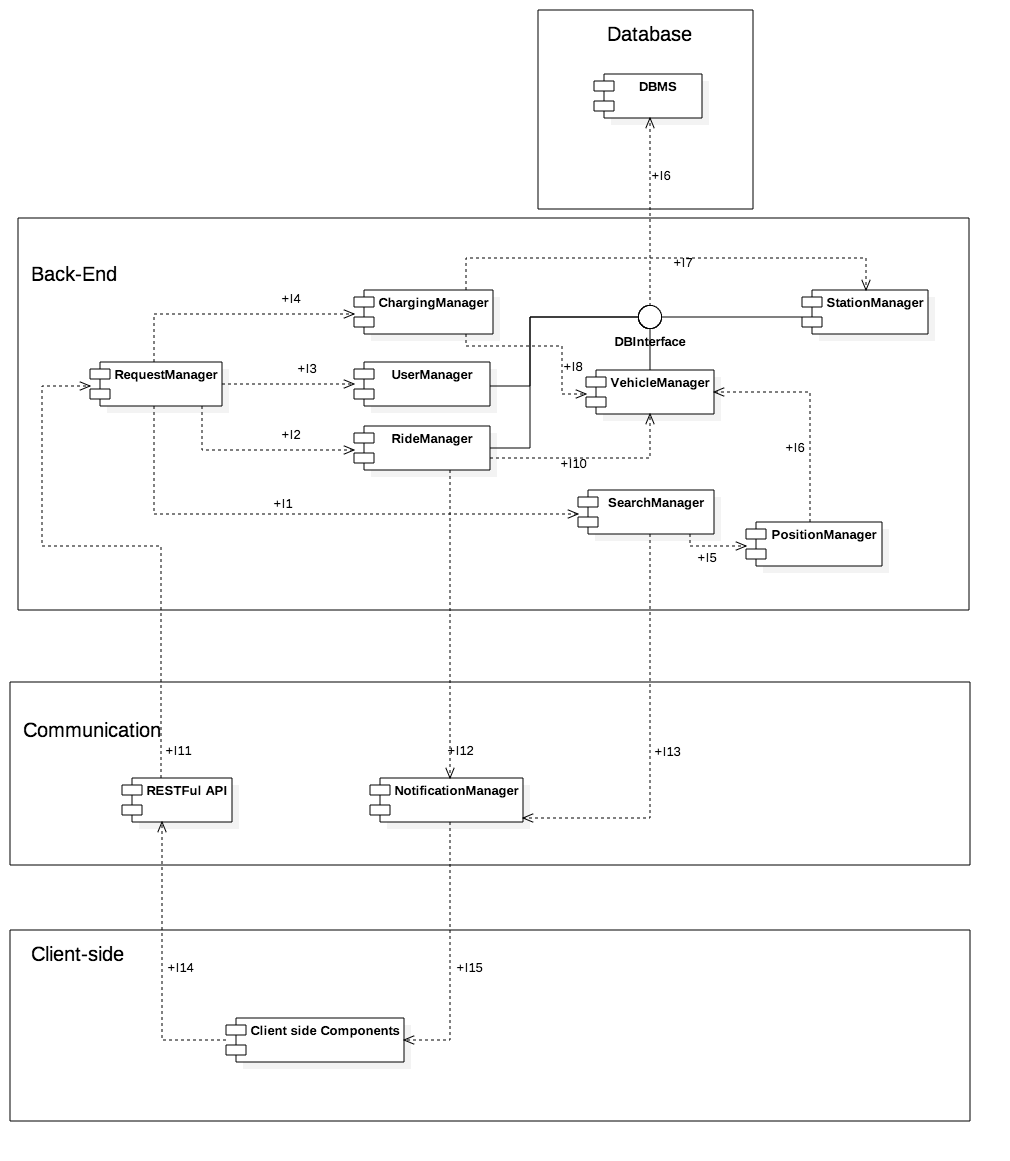
\includegraphics[scale=0.45]{Images/Diagram3.png}
\end{figure}
\FloatBarrier
\newpage

The following tables show the needed integration tests,highlighting their ID used in this document and the paragraph that describes them.\\
\FloatBarrier
\subsubsection{Back-End Tests}
\begin{table}[h]
\centering
\label{backTest}
\resizebox{\textwidth}{!}{%
\begin{tabular}{|l|l|c|}
\hline
\multicolumn{1}{|c|}{{\color[HTML]{333333} \textbf{ID}}} & \multicolumn{1}{c|}{{\color[HTML]{333333} \textbf{Integration Test}}} & {\color[HTML]{333333} \textbf{Paragraphs}} \\ \hline
1 & Request Manager $\rightarrow$ Search Manager & \ref{sub:IT1} \\ \hline
2 & Request Manager $\rightarrow$ Ride Manager & \ref{sub:IT2} \\ \hline
3 & Request Manager $\rightarrow$ User Manager & \ref{sub:IT3} \\ \hline
4 & Request Manager $\rightarrow$ Charging Manager & \ref{sub:IT4} \\ \hline
5 & Search Manager $\rightarrow$ Position Manager & \ref{sub:IT5} \\ \hline
6 & Position Manager $\rightarrow$ Vehicle Manager & \ref{sub:IT6} \\ \hline
7 & Charging Manager $\rightarrow$ Station Manager & \ref{sub:IT7} \\ \hline
8 & Charging Manager $\rightarrow$ Vehicle Manager & \ref{sub:IT8} \\ \hline
9 & Ride Manager $\rightarrow$ Vehicle Manager & \ref{sub:IT9} \\ \hline
10 & Database Interface $\rightarrow$ DBMS & \ref{sub:IT10} \\ \hline
\end{tabular}%
}
\caption{Back-End Tests Table}
\end{table}
\FloatBarrier

\subsubsection{Client-Server Tests}
\begin{table}[h]
\centering
\label{commTest}
\resizebox{\textwidth}{!}{%
\begin{tabular}{|l|l|c|}
\hline
\multicolumn{1}{|c|}{{\color[HTML]{333333} \textbf{ID}}} & \multicolumn{1}{c|}{{\color[HTML]{333333} \textbf{Integration Test}}} & {\color[HTML]{333333} \textbf{Paragraphs}} \\ \hline
11 & RESTful API $\rightarrow$ Request Manager & \ref{sub:IT11} \\ \hline
12 & Ride Manager $\rightarrow$ Notification Manager & \ref{sub:IT12} \\ \hline
13 & Search Manager $\rightarrow$ Notification Manager & \ref{sub:IT13} \\ \hline
14 & Notification Manager $\rightarrow$ Client-side components & \ref{sub:IT14} \\ \hline
15 & Client-side components $\rightarrow$ RESTful API & \ref{sub:IT15} \\ \hline
\end{tabular}%
}
\caption{Client-Server Tests Table}
\end{table}
\FloatBarrier
\newpage












